\section{Assignment 1}

\subsection{Implement the single-input single-output four-channel bilateral teleoperation architecture}

\begin{figure}[h]
\centering
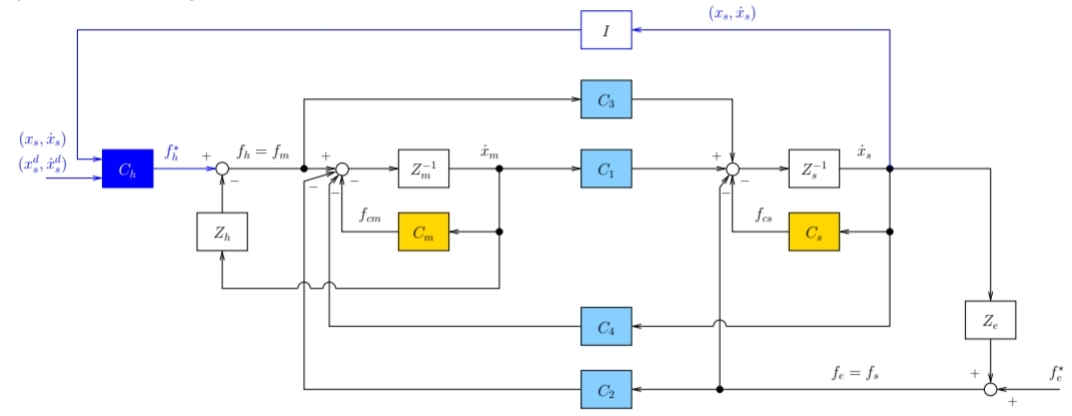
\includegraphics[keepaspectratio,width=0.9\textwidth]{4ch_arch}
\caption{SISO 4ch bilateral teleoperation architecture}
\end{figure}

The inner controllers for the robots are defined as follows:
\begin{equation*}
C_m=B_m+\frac{K_m}{s}\;\;\;\;\;\;C_s=B_s+\frac{K_s}{s}
\end{equation*}

To achieve perfect transparency, the coordination controllers must satisfy the following conditions:
\begin{align*}
\begin{cases}
C_1&=Z_s+C_s\\
C_2&=I\\
C_3&=I\\
C_4&=-(Z_m+C_m)
\end{cases}\;\;\;\;\text{with }Z_m=M_ms+D_m,\;Z_s=M_ss+D_s
\end{align*}

with $M_m=0.5,M_s=2,D_m=D_s=0$.

The human is modelled  with damping $B_h=1$ and stiffness $K_h=0$. The human intention is modelled with a PD controller with $K_P=2000$ and $K_D=50$. The master robot is controlled with a PD controller with $K_P=20$ and $K_D=10$. The slave robot is controlled with a PD controller with $K_P=4000$ and $K_D=500$.

The environment is modelled as a spring with  inertia $B_e=100$ and stiffness $K_e=200$.

The architecture is tested with a low-pass filtered step signal ($f_{lp}=0.5$Hz, $A=1$) and with a sinusoidal signal ($A=1$, $f=1$Hz), both in free motion ($x_e = 1.5$) and in contact ($x_e = 0.75$). The architecture is tested both with $D_m=D_s=0$ and $D_m=5,D_s=10$.

The architecture is modeled in simulink as follows:

\begin{figure}[H]
\centering
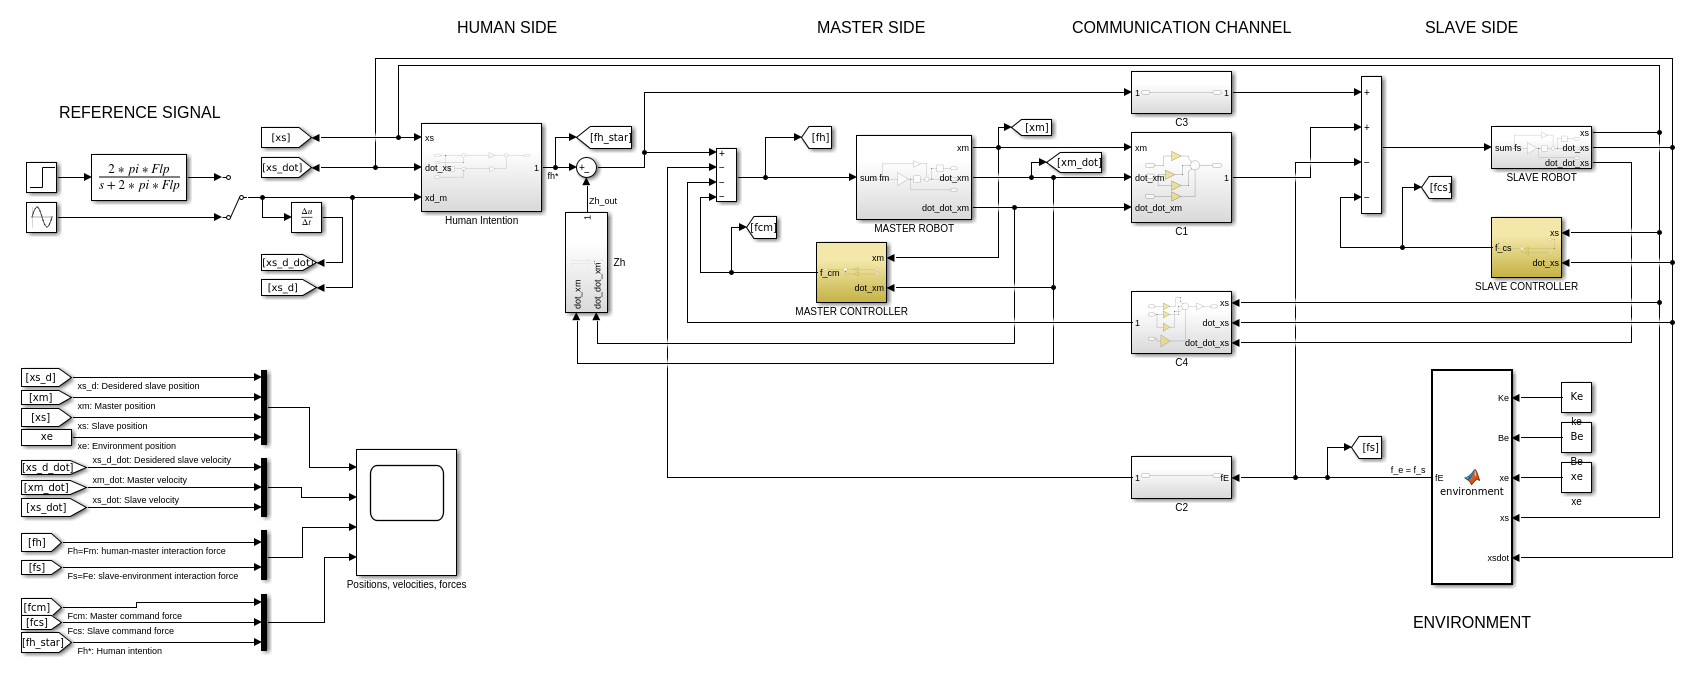
\includegraphics[keepaspectratio,width=0.85\textwidth]{4ch_simulink}
\caption{SISO 4ch bilateral teleoperation architecture - SIMULINK model}
\end{figure}

\newpage

\begin{figure}[H]
\begin{minipage}{0.5\textwidth}
\begin{figure}[H]
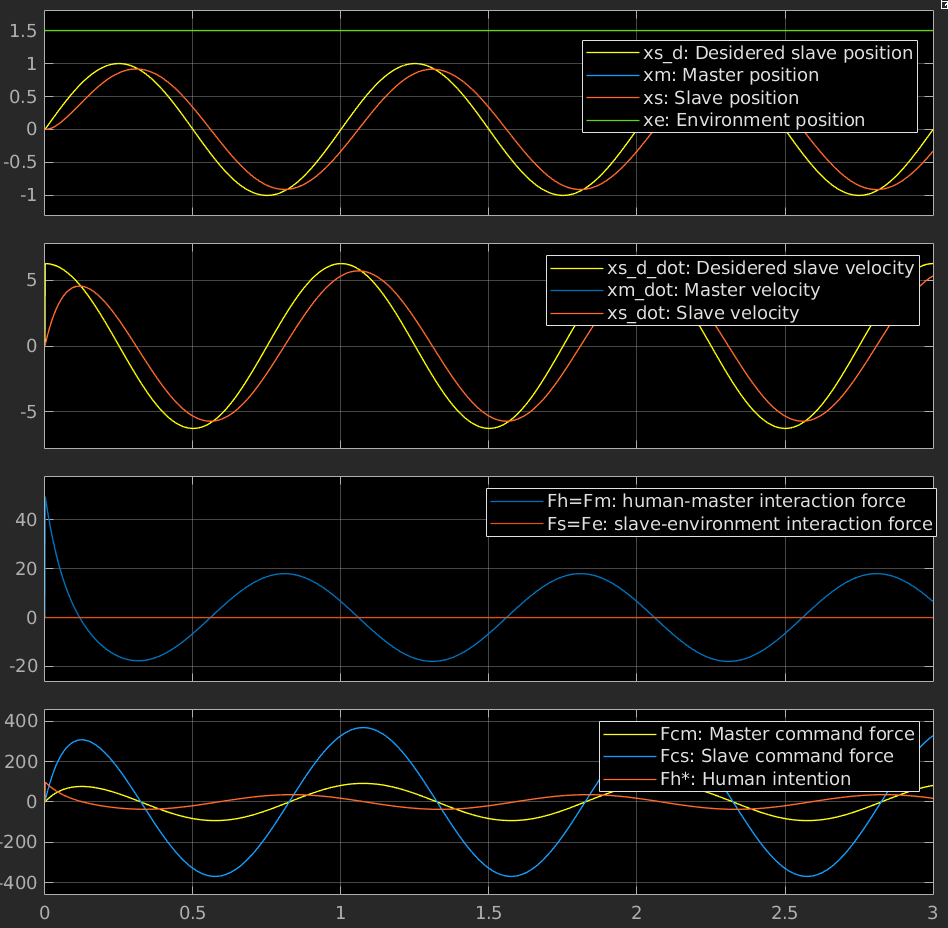
\includegraphics[keepaspectratio,width=\textwidth]{sin_free_nod}
\caption{Sinusoidal response in free motion\\ with $Dm=Ds=0$}
\label{fig:sin_free_nod}
\end{figure}
\begin{figure}[H]
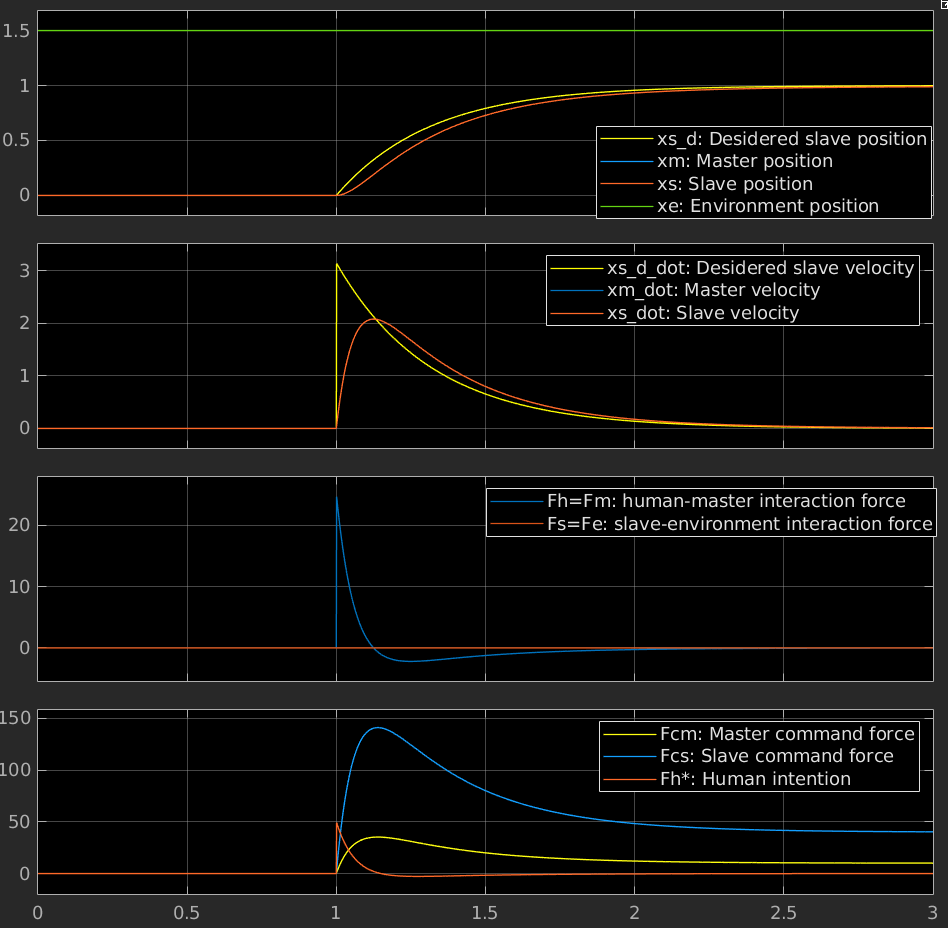
\includegraphics[keepaspectratio,width=\textwidth]{step_free_nod}
\caption{Step response in free motion with $Dm=Ds=0$}
\label{fig:step_free_nod}
\end{figure}
\end{minipage}
\begin{minipage}{0.5\textwidth}
\begin{figure}[H]
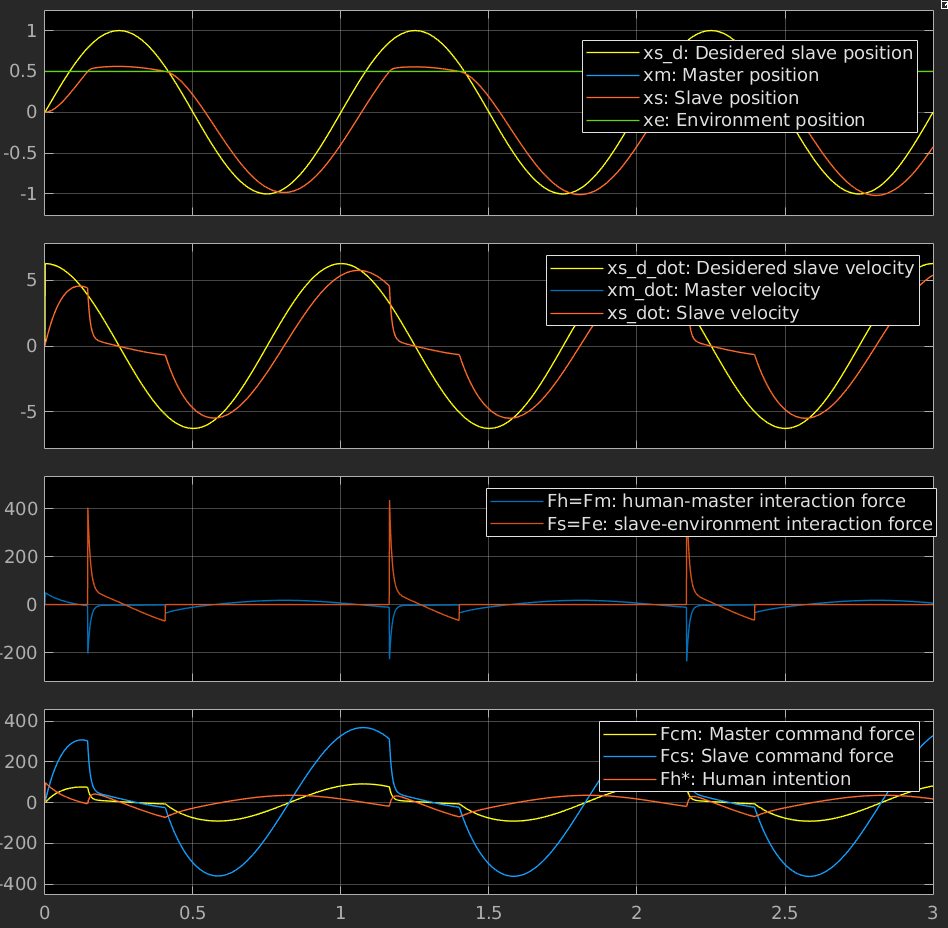
\includegraphics[keepaspectratio,width=\textwidth]{sin_contact_nod}
\caption{Sinusoidal response in contact\\ with $Dm=Ds=0$}
\label{fig:sin_contact_nod}
\end{figure}
\begin{figure}[H]
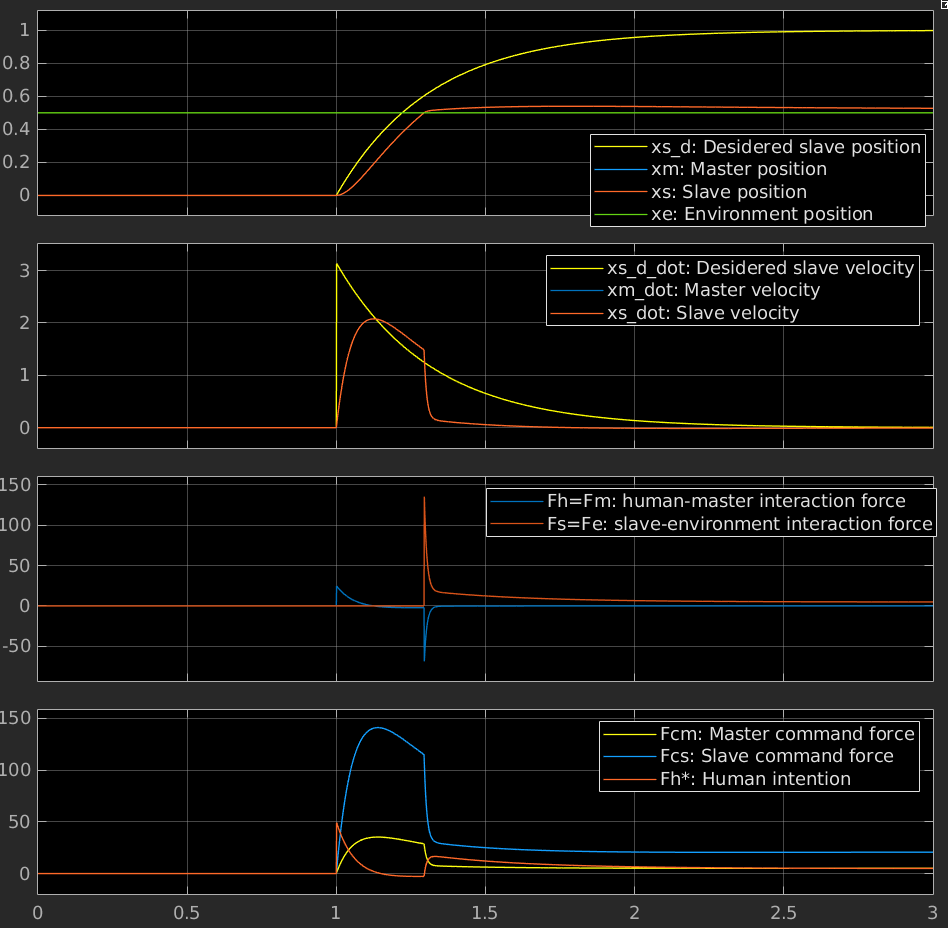
\includegraphics[keepaspectratio,width=\textwidth]{step_contact_nod}
\caption{Step response in contact with $Dm=Ds=0$}
\label{fig:step_contact_nod}
\end{figure}
\end{minipage}
\end{figure}

In both the sinusoidal and step reference cases, the trajectory is followed with some delay in free motion (figures \ref{fig:sin_free_nod} and \ref{fig:step_free_nod}). In contact (figures \ref{fig:sin_contact_nod} and \ref{fig:step_contact_nod}), once the slave reaches the environment there are sharp spikes in the force of both slave and master, and the trajectory is no longer followed during contact. In all cases, under the condition of perfect transparency, the slave and master robots positions are the same.

\newpage

\begin{figure}[H]
\begin{minipage}{0.5\textwidth}
\begin{figure}[H]
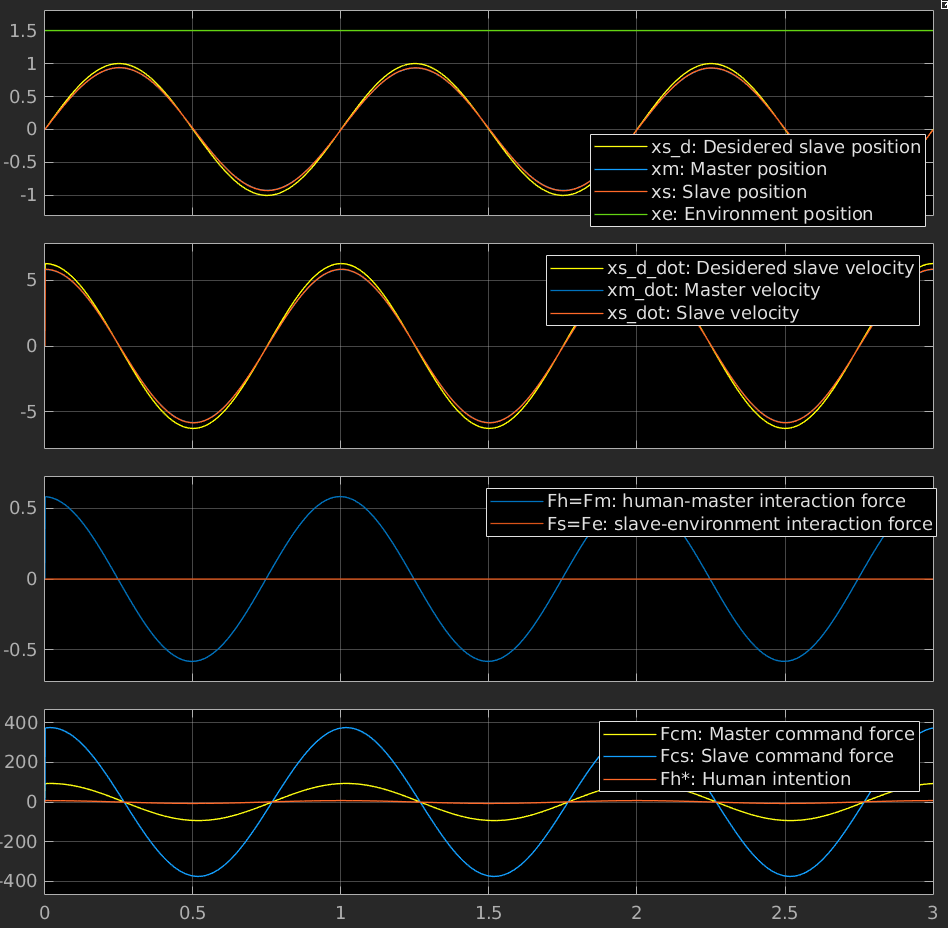
\includegraphics[keepaspectratio,width=\textwidth]{sin_free_d}
\caption{Sinusoidal response in free motion\\ with $Dm=5,Ds=10$}
\label{fig:sin_free_d}
\end{figure}
\begin{figure}[H]
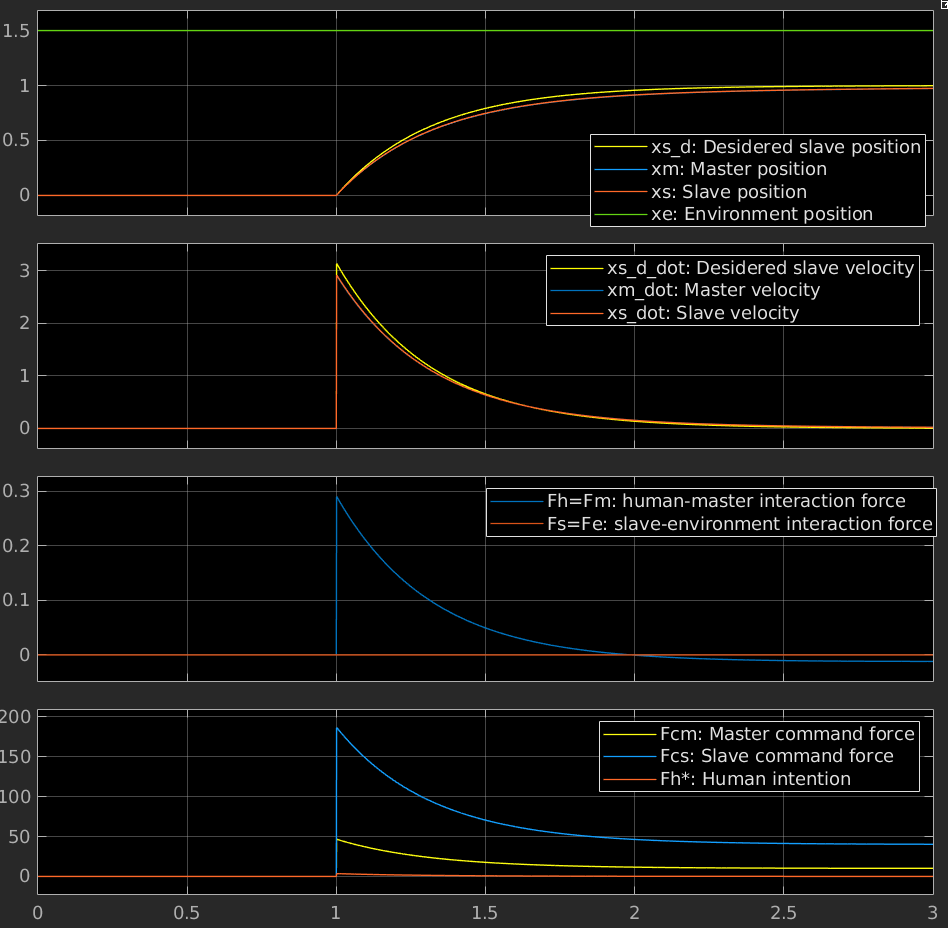
\includegraphics[keepaspectratio,width=\textwidth]{step_free_d}
\caption{Step response in free motion\\ with $Dm=5,Ds=10$}
\label{fig:step_free_d}
\end{figure}
\end{minipage}
\begin{minipage}{0.5\textwidth}
\begin{figure}[H]
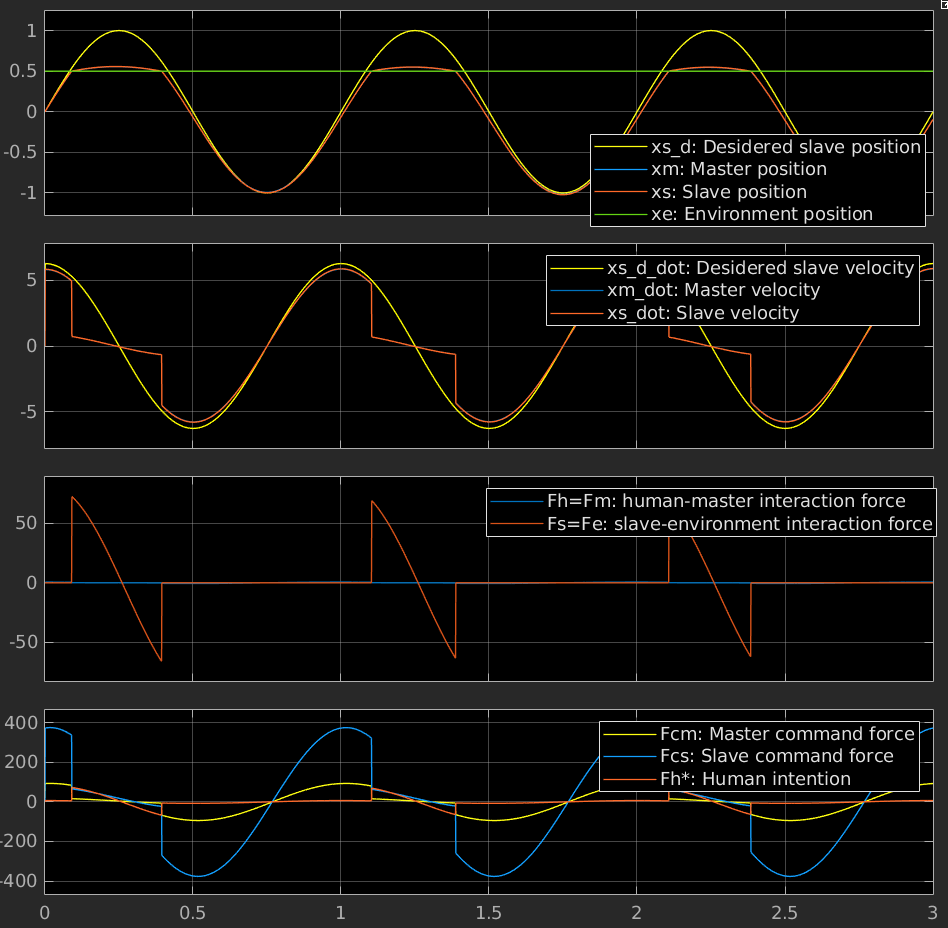
\includegraphics[keepaspectratio,width=\textwidth]{sin_contact_d}
\caption{Sinusoidal response in contact\\ with $Dm=5,Ds=10$}
\label{fig:sin_contact_d}
\end{figure}
\begin{figure}[H]
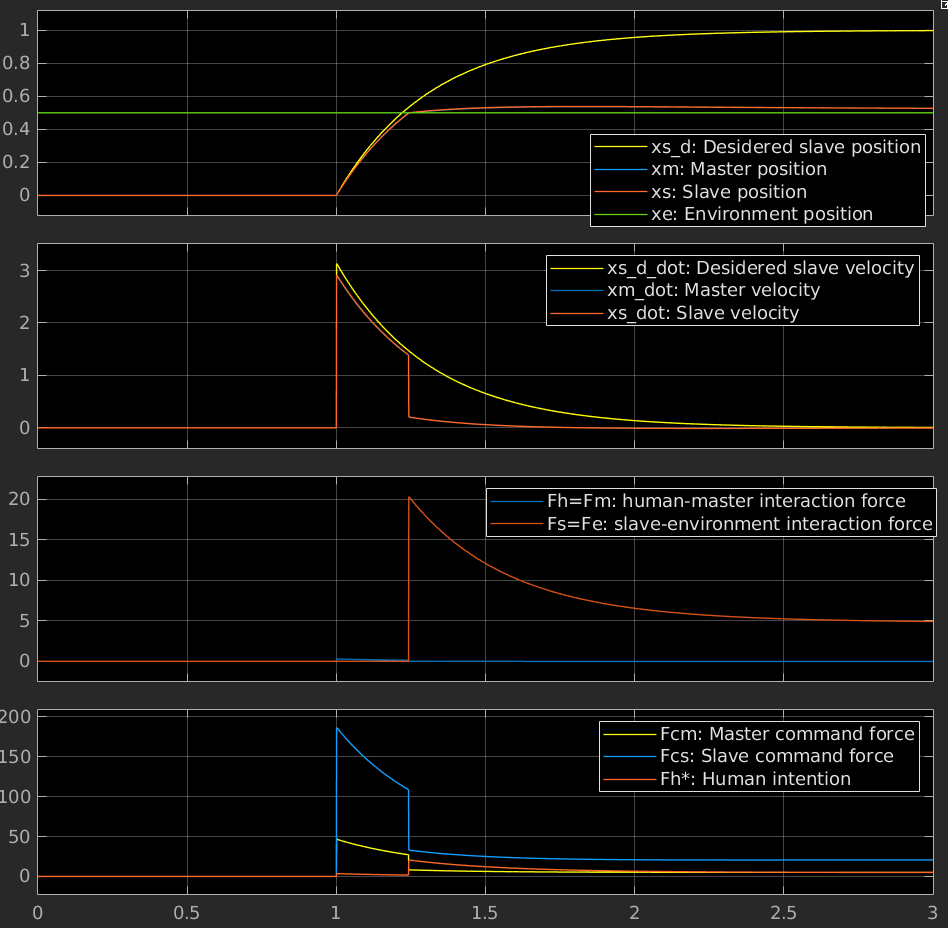
\includegraphics[keepaspectratio,width=\textwidth]{step_contact_d}
\caption{Step response in contact\\\hspace{\textwidth} with $Dm=5,Ds=10$}
\label{fig:step_contact_d}
\end{figure}
\end{minipage}
\end{figure}

Using damping values of $D_m=5,D_s=10$ improves the trajectory execution, both in the free motion (figures \ref{fig:sin_free_d} and \ref{fig:step_free_d}) and contact (figures \ref{fig:sin_contact_d} and \ref{fig:step_contact_d}) cases. Additionally the force spikes observed in the contact case are reduced.